% Name: Monoid laws
% Description: The associativity and unit laws of a monoid as string diagrams: merging three strands in either order gives the same result, and merging with the unit leaves a strand unchanged.
% Tags: string diagrams, monoid, associativity, unit, category theory

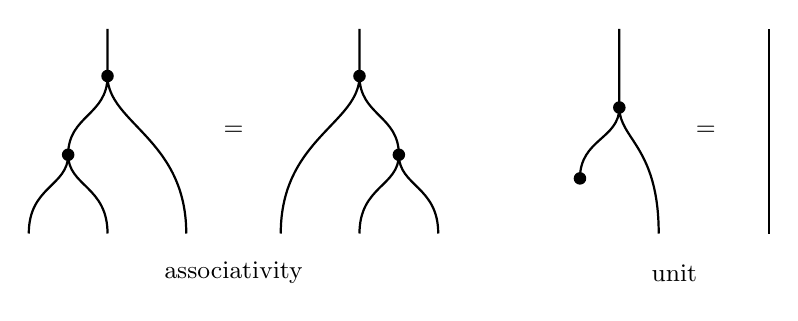
\begin{tikzpicture}[thick, every node/.style={font=\small}, dot/.style={circle, fill, inner sep=1.6pt}]
  % A merge: two strands in at the bottom, one out at the top, joined at a dot
  \draw (0,0) .. controls (0,0.6) and (0.5,0.6) .. (0.5,1) (1,0) .. controls (1,0.6) and (0.5,0.6) .. (0.5,1);
  \draw (0.5,1) .. controls (0.5,1.5) and (1,1.5) .. (1,2) (2,0) .. controls (2,1.2) and (1,1.4) .. (1,2) -- (1,2.6);
  \node[dot] at (0.5,1) {}; \node[dot] at (1,2) {};
  \node at (2.6,1.3) {$=$};
  \draw (4.2,0) .. controls (4.2,0.6) and (4.7,0.6) .. (4.7,1) (5.2,0) .. controls (5.2,0.6) and (4.7,0.6) .. (4.7,1);
  \draw (4.7,1) .. controls (4.7,1.5) and (4.2,1.5) .. (4.2,2) (3.2,0) .. controls (3.2,1.2) and (4.2,1.4) .. (4.2,2) -- (4.2,2.6);
  \node[dot] at (4.7,1) {}; \node[dot] at (4.2,2) {};
  % The unit law: a strand that starts at the unit dot, merged in, does nothing
  \draw (7,0.7) .. controls (7,1.2) and (7.5,1.2) .. (7.5,1.6) (8,0) .. controls (8,1.1) and (7.5,1.2) .. (7.5,1.6) -- (7.5,2.6);
  \node[dot] at (7,0.7) {}; \node[dot] at (7.5,1.6) {};
  \node at (8.6,1.3) {$=$};
  \draw (9.4,0) -- (9.4,2.6);
  \node at (2.6,-0.5) {associativity};
  \node at (8.2,-0.5) {unit};
\end{tikzpicture}
